\documentclass[dvipsnames,hidelinks,t]{beamer}

  % Enables the use of colour.
  \usepackage{xcolor}
  % Syntax high-lighting for code. Requires Python's pygments.
  \usepackage{minted}
  % Enables the use of umlauts and other accents.
  \usepackage[utf8]{inputenc}
  % Diagrams.
  \usepackage{tikz}
  % Settings for captions, such as sideways captions.
  \usepackage{caption}
  % Symbols for units, like degrees and ohms.
  \usepackage{gensymb}
  % Latin modern fonts - better looking than the defaults.
  \usepackage{lmodern}
  % Allows for columns spanning multiple rows in tables.
  \usepackage{multirow}
  % Better looking tables, including nicer borders.
  \usepackage{booktabs}
  % More math symbols.
  \usepackage{amssymb}
  % More math fonts, like mathbb.
  \usepackage{amsfonts}
  % More math layouts, equation arrays, etc.
  \usepackage{amsmath}
  % More theorem environments.
  \usepackage{amsthm}
  % More column formats for tables.
  \usepackage{array}
  % Adjust the sizes of box environments.
  \usepackage{adjustbox}
  % Better looking single quotes in verbatim and minted environments.
  \usepackage{upquote}
  % Better blank space decisions.
  \usepackage{xspace}
  % Better looking tikz trees.
  \usepackage{forest}
  % URLs.
  \usepackage{hyperref}
  % For plotting.
  \usepackage{pgfplots}
  
  % Various tikz libraries.
  % For drawing mind maps.
  \usetikzlibrary{mindmap}
  % For adding shadows.
  \usetikzlibrary{shadows}
  % Extra arrows tips.
  \usetikzlibrary{arrows.meta}
  % Old arrows.
  \usetikzlibrary{arrows}
  % Automata.
  \usetikzlibrary{automata}
  % For more positioning options.
  \usetikzlibrary{positioning}
  % Creating chains of nodes on a line.
  \usetikzlibrary{chains}
  % Fitting node to contain set of coordinates.
  \usetikzlibrary{fit}
  % Extra shapes for drawing.
  \usetikzlibrary{shapes}
  % For markings on paths.
  \usetikzlibrary{decorations.markings}
  % For advanced calculations.
  \usetikzlibrary{calc}
  
  % GMIT colours.
  \definecolor{gmitblue}{RGB}{20,134,225}
  \definecolor{gmitred}{RGB}{220,20,60}
  \definecolor{gmitgrey}{RGB}{67,67,67}
  
  % Change some style options.
  \usetheme{metropolis}
  % Tell minted to use the following colour scheme. 
  \usemintedstyle{manni}
  % Remove some of the vertical space after the title.
  \addtobeamertemplate{frametitle}{}{\vspace{-3mm}}
  % Change the default theme colours.
  \setbeamercolor{normal text}{fg=darkgray, bg=white}
  \setbeamercolor{alerted text}{fg=gmitred, bg=white}
  \setbeamercolor{example text}{fg=gmitblue, bg=white}
  \setbeamercolor{frametitle}{fg=gmitblue, bg=white}
  \setbeamercolor*{item}{fg=gmitblue}
  % Use a better math mode font.
  \usefonttheme[onlymath]{serif}
  % Don't display section pages.
  \metroset{sectionpage=none}
  % Change the default itemize bullets.
  \setbeamertemplate{itemize item}{\color{gray}--}
  % Change the position of left aligned math.
  %\setlength{\mathindent}{7mm}

  % An environment for displaying math in red, without lots of vertical space.
  \newcommand{\redmath}[1]{\vspace{-3mm} {\begin{center} \color{gmitred} $ #1 $ \end{center}} \vspace{-2mm}}

  % For displaying a blank character.
  \newcommand{\bl}{\underline{\hspace{2mm}}}

  % \citeurl can be used to a clickable short url to a slide as a reference.
  \renewcommand\footnoterule{}
  \newcommand{\citeurl}[1]{\let\thefootnote\relax\footnotetext{\tiny \textcolor{gmitgrey}{\href{http://#1}{#1}}}}
  \newcommand{\citeeg}[1]{\let\thefootnote\relax\footnotetext{\tiny \textcolor{gmitgrey}{#1}}}
  
  % Prevent minted from showing errors.
  \makeatletter
  \expandafter\def\csname PYGdefault@tok@err\endcsname{\def\PYGdefault@bc##1{{\strut ##1}}}
  \makeatother
  
  \begin{document}
    \title{Turing machines}
    \subtitle{}
    \author{ian.mcloughlin@gmit.ie}
    \date{}
  
    \begin{frame}
      \titlepage
    \end{frame}
  
    \begin{frame}{Visualisation}

  \begin{adjustbox}{max width={0.9\textwidth},center} 
    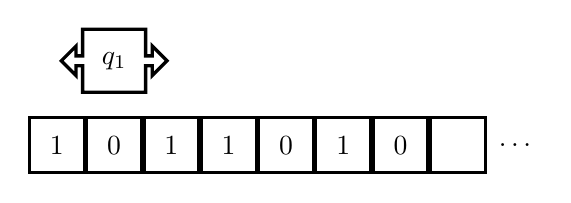
\begin{tikzpicture}
      \tikzstyle{every path}=[very thick]
      
      \edef\sizetape{0.7cm}
      \tikzstyle{tmtape}=[draw,minimum size=\sizetape]
      \tikzstyle{tmhead}=[arrow box,draw,minimum size=.8cm,arrow box arrows={east:.25cm, west:0.25cm}]
      
      \begin{scope}[start chain=1 going right,node distance=-0.15mm]
        \node [on chain=1,tmtape] {1};
        \node [on chain=1,tmtape] (input) {0};
        \node [on chain=1,tmtape] {1};
        \node [on chain=1,tmtape] {1};
        \node [on chain=1,tmtape] {0};
        \node [on chain=1,tmtape] {1};
        \node [on chain=1,tmtape] {0};
        \node [on chain=1,tmtape] {};
        \node [on chain=1,tmtape,draw=none] {$\ldots$};
      \end{scope}

      \node [tmhead,yshift=.7cm] at (input.north) (head) {$q_1$};
    \end{tikzpicture}
  \end{adjustbox}

  \vspace{1cm}

  \begin{adjustbox}{max width={0.9\textwidth},center} 
    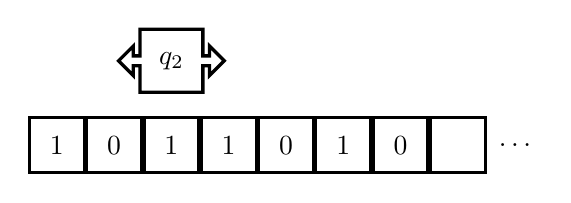
\begin{tikzpicture}
      \tikzstyle{every path}=[very thick]
      
      \edef\sizetape{0.7cm}
      \tikzstyle{tmtape}=[draw,minimum size=\sizetape]
      \tikzstyle{tmhead}=[arrow box,draw,minimum size=.8cm,arrow box arrows={east:.25cm, west:0.25cm}]
      
      \begin{scope}[start chain=1 going right,node distance=-0.15mm]
        \node [on chain=1,tmtape] {1};
        \node [on chain=1,tmtape] {0};
        \node [on chain=1,tmtape] (input) {1};
        \node [on chain=1,tmtape] {1};
        \node [on chain=1,tmtape] {0};
        \node [on chain=1,tmtape] {1};
        \node [on chain=1,tmtape] {0};
        \node [on chain=1,tmtape] {};
        \node [on chain=1,tmtape,draw=none] {$\ldots$};
      \end{scope}
      
      \node [tmhead,yshift=.7cm] at (input.north) (head) {$q_2$};
    \end{tikzpicture}
  \end{adjustbox}
\end{frame}

\begin{frame}{State Table}
  \begin{table}
    \centering
    \begin{tabular}{cc|ccc}
    \toprule
        State & Input & Write & Move & Next \\
    \midrule
        $q_0$ & $\sqcup$ & $\sqcup$ & L & $q_a$ \\
        $q_0$ & 0 & 0 & R & $q_0$ \\
        $q_0$ & 1 & 1 & R & $q_1$ \\
    \midrule
        $q_1$ & $\sqcup$ & $\sqcup$ & L & $q_f$ \\
        $q_1$ & 0 & 0 & R & $q_1$ \\
        $q_1$ & 1 & 1 & R & $q_0$ \\
    \bottomrule
    \end{tabular}
  \end{table}
  \begin{center}
    $\delta(q_i, \gamma_n) \rightarrow (q_j, \gamma_m, L/R)$
  \end{center}
\end{frame}


\begin{frame}{Running an input}
  \begin{topdisp}
    $$\textrm{Tape input:} \  101101$$
  \end{topdisp}
  \begin{center}
    \setlength{\tabcolsep}{3pt}
    \begin{tabular}{ccccccccccccccc}
      $q_0$ & 1 &       & 0 &       & 1 &       & 1 &       & 0 &       & 1 &       &          &       \\
            & 1 & $q_1$ & 0 &       & 1 &       & 1 &       & 0 &       & 1 &       &          &       \\
            & 1 &       & 0 & $q_1$ & 1 &       & 1 &       & 0 &       & 1 &       &          &       \\
            & 1 &       & 0 &       & 1 & $q_0$ & 1 &       & 0 &       & 1 &       &          &       \\
            & 1 &       & 0 &       & 1 &       & 1 & $q_1$ & 0 &       & 1 &       &          &       \\
            & 1 &       & 0 &       & 1 &       & 1 &       & 0 & $q_1$ & 1 &       &          &       \\
            & 1 &       & 0 &       & 1 &       & 1 &       & 0 &       & 1 & $q_0$ & \bl &       \\
            & 1 &       & 0 &       & 1 &       & 1 &       & 0 &       & 1 &       & \bl & $q_a$
    \end{tabular}
  \end{center}
  \vspace{6mm}
  \begin{topdisp}
    $$\textrm{Tape output:} \  101101$$
    $$\textrm{Final state:} \  q_a \textrm{ (the accept state)}$$
  \end{topdisp}

\end{frame}


\begin{frame}{Outcomes}
  Running a Turing machine on a given tape input has two effects.

  \begin{alertblock}{Tape content}
    Sometimes we're interested in what is left on the tape when the Turing machine finishes. Even for Turing machines that run forever, we can be interested in the tape output. Turing's examples focused on this.
  \end{alertblock}

  \begin{alertblock}{Accept or Fail}
    We are also interested in whether or not the Turing machine accepts the given tape input (by ending in the accept state) or rejects it (by ending in the reject state). There is a third possibility: the machine doesn't stop.
  \end{alertblock}
\end{frame}


\begin{frame}{Notation}
  \begin{topdisp}
    $$M = (Q, \Sigma, \Gamma, \delta , q_0, q_a, q_r )$$
  \end{topdisp}
  \begin{description}[aaaaaaaa]
    \item[$Q$] Set of states (finite)
    \item[$\Sigma$] Input alphabet, subset of $\Gamma \setminus \{ \sqcup \} $
    \item[$\Gamma$] Tape alphabet (finite)
    \item[$\sqcup$] Blank symbol, element of $\Gamma$
    \item[$\delta$] Transition function, $\delta: Q \times \Gamma \rightarrow Q \times \Gamma \times \{L,R\}$
    \item[$q_0$] Start state, $\in Q$
    \item[$q_a$] Accept state, $\in Q$
    \item[$q_r$] Reject state, $\in Q$, $\neq q_a$
  \end{description}
\end{frame}


\begin{frame}{The blank symbol}
  \begin{description}
    \setlength\itemsep{4mm}
    \item[\bl] is generally the only difference between the tape alphabet and the input alphabet.
    \item[Some] definitions of Turing machines permit other symbols in the difference.
    \item[Empty cells] of the tape in the machine are said to contain the blank symbol.
    \item[Important] because the blank symbol marks the end of the input on the tape, so blank can't form part of the input.
  \end{description}
\end{frame}


\begin{frame}{Alphabets}

  \begin{description}[Alphabets]
    \setlength\itemsep{4mm}
    \item[Sets] are collections of objects. An object is either in the set or not, and elements are distinct.
    \item[Alphabets] are sets, strings are tuples over alphabets.
    \item[$\epsilon$] is the empty string.
    \item[$A^*$] is the set of all strings over alphabet A, including $\epsilon$.
    \item[$|w|$] denotes the length of a string $w$, e.g. $|001110|=6$.
  \end{description}
\end{frame}

\begin{frame}{Strings}
  \begin{alertblock}{Examples}
    The following are examples of strings over the alphabet $\{0,1\}$:
    $$100110, 111, 0, \epsilon, 0101010, 1, 11$$
  \end{alertblock}
\metroset{block=transparent}
\begin{alertblock}{Single character strings}
Note the distinction between a symbol in an alphabet and the string containing a single symbol.
They look the same, but one is a symbol and one is a string. 
This is akin to the distinction in C between the character \mintinline{c}{'a'} and the string literal \mintinline{c}{"a"}.
\end{alertblock}
\end{frame}


\begin{frame}{Decidable languages}
  \begin{description}
    \setlength\itemsep{4mm}
    \item[Language] is a set of strings.
    \item[TM] accepts a subset of $\Sigma^*$, the language of the TM.
    \item[Halting] -- a TM will accept an input, reject it, or never halt.
    \item[Decider] -- a TM that halts on all inputs \emph{decides} its language.
    \item[Decidable] language -- some TM decides it.
  \end{description}
\end{frame}



\begin{frame}{Turing's Second Example}
  \begin{exampleblock}{Turing's own words\ldots}
    As a slightly more difficult example we can construct a machine to compute the sequence $001011011101111011111\ldots$.
    The machine is to be capable of five $m$-configurations, viz. $\mathfrak{o}$, $\mathfrak{q}$, $\mathfrak{p}$, $\mathfrak{f}$, $\mathfrak{b}$ and of printing $e$, $x$, $0$, $1$.
    The first three symbols on the tape will be $ee0$; the other figures follow on alternate squares.
    On the intermediate squares we never print anything but $x$.
    These letters serve to keep the place for us and are erased when we have finished with them.
    We also arrange that in the sequence of figures on alternate squares there shall be no blanks.
  \end{exampleblock}
  \citeurl{www.cs.virginia.edu/~robins/Turing\_Paper\_1936.pdf}
\end{frame}



\begin{frame}{Turing's second example: state table}
  \vspace{-4mm}
  \begin{table}
    \resizebox{\textwidth}{!}{
      \centering
      \begin{tabular}{ccp{7cm}c}
        \toprule
        \textbf{m-config.}  & \textbf{symbol}  & \textbf{operations} & \textbf{final m-config.} \\
        \midrule
        $\mathfrak{b}$ & & $Pe,R,Pe,R,P0,R,R,P0,L,L$  & $\mathfrak{o}$ \\
        \midrule
        \multirow{2}{*}{$\mathfrak{o}$} & $1$ & $R,Px,L,L,L$ & $\mathfrak{o}$ \\
        & 0 & & $\mathfrak{q}$ \\
        \midrule
        \multirow{2}{*}{$\mathfrak{q}$} & Any (0 or 1) & $R,R$ & $\mathfrak{q}$ \\
        & None & $P1,L$ & $\mathfrak{p}$ \\
        \midrule
        \multirow{3}{*}{$\mathfrak{p}$} & x & $E,R$ & $\mathfrak{q}$ \\
        & e & R & $\mathfrak{f}$ \\
        & None & $L,L$ & $\mathfrak{p}$ \\
        \midrule
        \multirow{2}{*}{$\mathfrak{f}$} & Any & $R,R$ & $\mathfrak{f}$ \\
        & None & $P0,L,L$ & $\mathfrak{o}$ \\
        \bottomrule
      \end{tabular}
    }
  \end{table}
\end{frame}
 
  \end{document}